\documentclass[10pt,journal,compsoc]{IEEEtran}
\usepackage[T1]{fontenc}
\usepackage{graphicx}
\usepackage{amsmath,amssymb}
\usepackage{booktabs,array,tabularx,multirow}
\usepackage{microtype}
\usepackage[nocompress]{cite}
\usepackage{url}
\usepackage{xcolor}
\definecolor{ASVblue}{HTML}{3F6C9B}
\definecolor{ASVochre}{HTML}{B8753B}
\definecolor{ASVochreText}{HTML}{8C552A}
\definecolor{ASVgreen}{HTML}{4F7F5F}
\definecolor{ASVgray}{HTML}{6F6F6F}
\definecolor{ASVrule}{HTML}{D4D7D9}
\usepackage[hidelinks,hypertexnames=false]{hyperref}
\usepackage{tikz}
\usetikzlibrary{arrows.meta,positioning,fit,calc}
\usepackage{enumitem}
\usepackage{needspace}
\newcolumntype{Y}{>{\raggedright\arraybackslash}X}
\newcolumntype{L}[1]{>{\raggedright\arraybackslash}p{#1}}
\newcommand{\bit}{\mathrel{\equiv_{\mathrm{bits}}}}
\newcommand{\Simple}{\textsc{Simple}}
\newcommand{\Local}{\textsc{Local}}
\newcommand{\tighttable}{\renewcommand{\arraystretch}{1.10}\setlength{\tabcolsep}{4pt}}
\newcommand{\evidence}[1]{\textsf{#1}}
\setlist[enumerate]{leftmargin=*,itemsep=2pt,topsep=3pt}
\setlist[itemize]{leftmargin=*,itemsep=1pt,topsep=3pt}
\interdisplaylinepenalty=2500
\hyphenation{CUDA Vulkan pre-fill kernel back-end back-ends micro-batch}
\hypersetup{pdftitle={Reference-Compatible Parallel Execution for Quantized LLM Inference},pdfauthor={Chengzhan Li},pdfsubject={Reference-derived phase plans for quantized language-model execution}}
% Use the class's body size, leading, margins and column width.
\setlength{\textfloatsep}{11pt plus 2pt minus 2pt}
\setlength{\dbltextfloatsep}{11pt plus 2pt minus 2pt}
\setlength{\floatsep}{9pt plus 2pt minus 2pt}
\setlength{\dblfloatsep}{9pt plus 2pt minus 2pt}
\setcounter{topnumber}{3}
\setcounter{dbltopnumber}{2}
\renewcommand{\topfraction}{.90}
\renewcommand{\dbltopfraction}{.90}
\renewcommand{\textfraction}{.08}
\renewcommand{\floatpagefraction}{.80}
\renewcommand{\dblfloatpagefraction}{.80}
\raggedbottom

\newcommand{\StrongSTwoRows}{%
Q4\_K & q4 & 0.7370 & 0.9693 & [0.9576, 0.9885] \\
Q4\_K & q32 & 0.4731 & 0.6929 & [0.6803, 0.7029] \\
Q6\_K & q4 & 0.8205 & 0.9903 & [0.9624, 1.0102] \\
Q6\_K & q32 & 0.5829 & 0.7954 & [0.7473, 0.8708] \\
}



\newcommand{\ApplicationRows}{%
Qwen3-8B & 2.7274 & 2.6898 & 2.7287 & 2.6913 & 2.2726 & 2.2269 \\
Qwen3-14B & 4.6298 & 4.6022 & 4.6291 & 4.6028 & 3.4643 & 3.4268 \\
Llama-8B & 2.8879 & 2.8516 & 2.8874 & 2.8515 & 2.5631 & 2.5230 \\
}
\newcommand{\FactorRows}{%
8B & L/W; loop4 fixed & 0.997913 & [0.995370, 0.999576] \\
8B & L/W; packed fixed & 0.998717 & [0.995953, 1.000570] \\
8B & P/L4; W fixed & 0.983648 & [0.980236, 0.988654] \\
8B & P/L4; L fixed & 0.984440 & [0.981228, 0.989391] \\
14B & L/W; loop4 fixed & 0.996957 & [0.994726, 0.999092] \\
14B & L/W; packed fixed & 0.998881 & [0.997093, 1.000227] \\
14B & P/L4; W fixed & 0.990130 & [0.988351, 0.992804] \\
14B & P/L4; L fixed & 0.992041 & [0.990754, 0.993985] \\
}
\newcommand{\QThreeTwoRows}{%
\texttt{W\_REF1L\_M} & 124.182883 & 7.7614 & 343.310 & 425.997 \\
\texttt{W\_REF1G\_M} & 117.208239 & 7.3255 & 329.630 & 409.576 \\
\texttt{L\_REF1L\_M} & 124.100017 & 7.7563 & 344.139 & 428.399 \\
\texttt{L\_REF1G\_M} & 117.143582 & 7.3215 & 328.455 & 412.088 \\
\texttt{W\_REF1L\_D4} & 147.748374 & 9.2343 & 396.385 & 478.532 \\
\texttt{L\_REF1G\_D4} & 133.543739 & 8.3465 & 365.014 & 455.562 \\
}
\newcommand{\QEightRows}{%
W-L4-k3 & 185.311926 & 1.447749 \\
W-L4-k7 & 210.950040 & 1.648047 \\
W-P-k3 & 183.631913 & 1.434624 \\
W-P-k7 & 209.005981 & 1.632859 \\
L-L4-k3 & 183.035577 & 1.429965 \\
L-L4-k7 & 209.736406 & 1.638566 \\
L-P-k3 & 183.366590 & 1.432551 \\
L-P-k7 & 208.263503 & 1.627059 \\
}
\newcommand{\QEightSecondaryRows}{%
W-P-k7 / W-L4-k7 & 0.990784 & [0.981234, 1.000085] \\
L-P-k7 / L-L4-k7 & 0.992977 & [0.981103, 1.007912] \\
L-L4-k7 / W-L4-k7 & 0.994247 & [0.983947, 1.004513] \\
L-P-k7 / W-P-k7 & 0.996448 & [0.985822, 1.009280] \\
}

\newcommand{\AmperePilotRows}{%
Whole / loop4 & 12.039 & 13.824 \\
Whole / packed & 11.897 & 13.598 \\
Local / loop4 & 11.997 & 13.800 \\
Local / packed & 11.879 & 13.549 \\
}

\begin{document}
\title{Reference-Compatible Parallel Execution for Quantized LLM Inference}
\author{Chengzhan Li\IEEEcompsocitemizethanks{\IEEEcompsocthanksitem C. Li is with the University of Electronic Science and Technology of China, Chengdu, China. E-mail: chengzhan.li@std.uestc.edu.cn.}}
\markboth{REFERENCE-COMPATIBLE PARALLEL EXECUTION}{}
\IEEEtitleabstractindextext{\begin{abstract}Increasing query width during prompt processing or speculative verification can change a quantized language model's numerical behavior. We study how to reorganize this work while preserving a fixed deployment's outputs and state. Native operand-replay experiments show that a causal mask does not determine attention arithmetic: extending a physical key--value (KV) range can change the result even when the added probabilities are exactly zero. Query width can also change activation quantization, reduction organization and device placement. Producer history and output ownership connect these effects across inference phases. We use these findings to construct reference-derived execution plans. The runtime derives compatible query groups from live cache geometry, places cuts around whole graphs or within attention, and exposes independent arithmetic groups to the GPU while retaining each group's reference computation. One resident owner preserves requested outputs and the committed frontier. CUDA and Vulkan implementations cover Qwen, Llama and SmolLM2, including mixed Q4/Q6 quantization at 32B. Compatible speculative applications reduce Linux/A5000 resident service time by 11.52\%--25.54\% against the fastest measured fixed target-only controls. Balanced experiments attribute 0.80\%--1.64\% to Q8 projection packing; the smaller contribution of local cuts follows the available cache-boundary geometry. Complete-request measurements identify when parallel execution improves service.
\end{abstract}
\begin{IEEEkeywords}Parallel inference, quantized language models, numerical compatibility, execution planning, speculative decoding.\end{IEEEkeywords}}
\maketitle
\IEEEdisplaynontitleabstractindextext
\section{Introduction}
\label{sec:intro}
An established quantized language-model deployment supplies a numerical reference: prompt processing creates its key--value (KV) state, and continuation produces its target vectors and tokens. A prompt provides many known query rows; speculative decoding proposes several continuation tokens for one target verification~\cite{leviathan2023,chen2023}. The optimization problem is to process this known-query work faster while preserving the outputs and state on which regression tests and stateful continuations depend.

A four-query Llama execution illustrates the difficulty (Fig.~\ref{fig:extent_intervention}). Its single-query reference consumed physical KV extents of 768, 768, 768 and 1024 entries; the wider call consumed 1024 for every query. Visible attention inputs and probability prefixes agreed, and the added probabilities were exactly zero, yet the attention output differed. Cropped and padded native replays reproduced the two results. Target vectors diverged before emitted tokens did. Matching the model, positions and causal mask therefore does not determine the runtime's numerical computation.

\begin{figure*}[t]
\centering
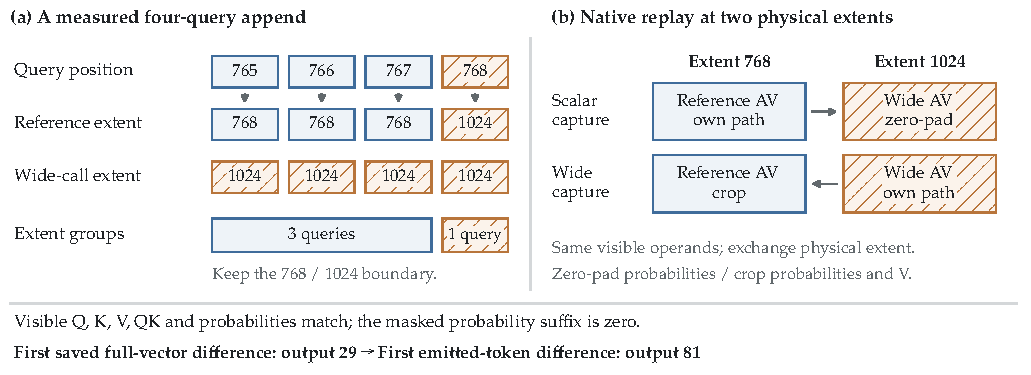
\includegraphics[width=\textwidth]{figures/extent_intervention.pdf}
\caption{Physical-range intervention on the CUDA Llama failure. The four queries require reference extents $[768,768,768,1024]$, while the unsplit call uses 1024. Replays of the first affected query exchange the cropped and padded attention--value (AV) ranges with the consumer query width fixed. The outputs follow the physical range despite identical visible operands and an exactly zero masked probability suffix. The first full-vector discrepancy precedes the first emitted-token discrepancy.}
\label{fig:extent_intervention}
\end{figure*}

Further native interventions identify width-dependent activation quantization, reduction organization and CPU/GPU placement. Producer and commit-state studies show how these requirements extend across calls: compatible arithmetic needs compatible incoming state, and its resulting vectors must remain associated with the retained logical prefix.

We construct a \emph{reference-derived phase plan} from a backend arithmetic recipe and live cache geometry. Source analysis and native operand replays establish the recipe offline. At each call, the planner reads occupancy, physical head, capacity and padding to assign each query its reference extent, then groups adjacent queries with compatible requirements. Whole-graph execution places cuts around the complete computation; local execution confines them to attention and keeps projection and feed-forward work wider. Whole execution also provides the strong simple control for evaluating local cuts.

A separate choice exposes projection parallelism. On the affected CUDA Q8 path, independent groups retain the native four-column computation and run as channels of one GPU operation. A mixed Q4\_K/Q6\_K extension uses scalar-column arithmetic instead. These arithmetic groups differ from the query groups defined by physical KV extent. The executor owns requested outputs by logical row and maintains the committed frontier on one resident target/KV state. Prefill, continuation and verification share this interface while retaining their phase-specific numerical behavior.

Batch-invariant operators control reduction choices~\cite{thinkingmachines}; arithmetic reconstruction and compiler enforcement preserve existing library behavior~\cite{taming}; deterministic engines connect kernel properties with state invariants~\cite{vosti}. Fixed-shape schedules and verified speculation provide system designs for consistent execution~\cite{corun,llm42}. We connect these numerical concerns to a quantized deployment's physical cache range and phase state to determine where known-query work can be combined.

The evaluation first checks full target vectors and active state, then separates the effects of cut placement and arithmetic packing. The implementations cover CUDA and Vulkan, three model families and a 32B mixed-quantization path. In balanced Linux/A5000 experiments, Q8 packing contributes 0.80\%--1.64\%; the contribution of local cuts is smaller because most natural verification calls do not cross a physical boundary. Compatible speculative applications reduce resident service time by 17.21\%, 25.54\% and 11.52\% for Qwen3-8B, Qwen3-14B and Llama-8B against their fastest measured fixed target-only controls. Those application gains include speculation itself. Equal-work and live-request experiments further show why a cheaper wider target call can still produce a slower request when it induces more draft and verification work.

The paper makes two contributions: native interventions identify the physical, arithmetic and state requirements of wider execution, and an execution method derives query cuts, parallelizes independent arithmetic groups and composes calls through explicit output and state ownership. Numerical validation and controlled service measurements evaluate the resulting implementation.

\section{Why Batching Changes Results}
\label{sec:reference}
\subsection{A masked suffix changes attention}
The CUDA Llama reference processes continuation queries singly. At one four-query append, positions 765--768 require physical KV extents $[768,768,768,1024]$; an unsplit batch uses 1024 throughout. The first saved full target-vector difference occurs at generated-output index 29, whereas the first emitted-token difference occurs at index 81~\cite{records}. Inspecting only the divergent token would therefore start from a state that had already accumulated earlier discrepancies.

Captures at the first affected attention computation show identical visible query (Q), key (K), value (V), query--key (QK) and softmax probability prefixes. The masked probability suffix is exactly zero. We then replay the native attention--value (AV) aggregation operator with captured operands, keeping the consumer query width at one. Cropping the wide execution's probability and V ranges to 768 reproduces the reference AV output. Padding the reference probability range with zeros and supplying the corresponding 1024-entry V range reproduces the wide output. Own-path replays reproduce their respective captures. These bidirectional interventions isolate the physical attention range as a numerical execution dependency (Fig.~\ref{fig:extent_intervention}).



The physical range is thus part of the operator's numerical descriptor, including entries with zero attention mass. A Vulkan companion exposes a related dependency: changing the extent also changes contiguity and matvec dispatch. That intervention identifies their combined physical effect, which the backend recipe must preserve.

\subsection{Query width selects arithmetic and placement}
Query width also changes numerical choices outside attention. On an affected Vulkan Q8-weight path, a scalar operation consumes F32 activations, while a wider operation selects Q8\_1 activation quantization. Retaining the F32 path repairs that projection mismatch. In the Llama companion, this repair makes the emitted tokens agree while 99 committed full target vectors still differ. Applying the physical-prefix repair removes the remaining discrepancies~\cite{records}. Activation arithmetic and attention extent are separate requirements of the same execution.

On CUDA, the affected Q8 projection uses a small-column quantized matrix--vector (MMVQ) specialization. Traces for four and eight query columns show the same Q8\_1 input-quantizer kernel but different MMVQ launch organizations. Source inspection identifies four reduction warps at four columns and two at eight. Native replays with actual model operands match the scalar reference for the small-column path and diverge for the wider path~\cite{records}. This gives a useful unit of parallel work: preserve the four-column computation and expose several independent groups without selecting the eight-column reduction.

Placement also matters. In a partially offloaded Qwen deployment, increasing width moves K normalization and rotary position embedding (RoPE) from CPU to CUDA. Native RoPE replays with the same normalized K operands reproduce the output of the selected placement~\cite{records}. A compatible implementation must retain the reference scheduling decision where it affects arithmetic. The backend recipe therefore records activation types, reduction organization, placement, strides and dispatch conditions.

\subsection{Producer history and logical state connect the calls}
The prompt \emph{producer} creates the incoming KV cache and initial target vector. In a controlled Vulkan experiment, exchanging the producer changes both the serialized KV and the complete initial target vector on all eight tested inputs. On two long inputs, either producer followed by scalar continuation reaches the reference token endpoint, but the parallel consumers reach that endpoint after only one producer~\cite{records}. Scalar endpoint agreement therefore does not establish interchangeable producer state.

The reference binds producer semantics by phase. Our CUDA reference uses physical microbatch one with the original prompt caller and last-only output request. Candidate prefill can regroup these known rows when its outputs and state preserve that producer's result. The resident Vulkan plan retains the original physical microbatch 128 and outer prompt chunks, then selects a compatible continuation recipe.

State must also survive the boundary after a call. Verification may materialize several proposed tokens and retain only an accepted prefix. Its last physical output buffer can then belong to a rejected row instead of the retained frontier. A correction or bonus token can be emitted before it is materialized, and a generation cap or end-of-generation stop can leave that token pending. The executor must own requested vectors by logical row and update the active KV, frontier and pending-token record together.

\subsection{The resulting execution target}
These observations define what is fixed before optimization. A deployment reference $R_d$ includes model and tokenizer bytes, formatting, numerical modules, device placement, KV type and capacity, producer calls, requested outputs, sampling and stopping behavior. The candidate $F_d$ changes the organization of known-query work under that reference.

For a materialized token prefix $x$, let $\ell^R(x)$ be its full binary32 target vocabulary vector and $K^R(x)$ its active KV in canonical logical order. The target relation at an observed state boundary is
\begin{equation}
 \ell^F(x)\bit\ell^R(x),\qquad K^F(x)\bit K^R(x),
 \label{eq:contract}
\end{equation}
together with matching logical positions, frontier, pending token and termination behavior. Equality compares complete values without a tolerance; unused storage is outside the active state.

Speculative verification also requests vectors on branches that may later be rejected. For each such vector, an independent reference follows the same prefix after the original producer. A separate autonomous reference supplies the emitted-token and stopping endpoint. The draft may propose different tokens; compatibility concerns the target computations on the prefixes actually evaluated.

\section{Reference-Compatible Execution}
\label{sec:method}
\subsection{Derive query groups from live cache geometry}
A backend recipe specifies the reference-compatible activation and weight types, reduction organization, placement, supported shapes and strides, and output layout. Source analysis, own-path replay and cross-path comparisons on captured model operands establish this recipe offline. At runtime, descriptor guards select it from the current phase and operator metadata. The planner then groups queries whose live geometry allows them to share that recipe.

For the supported dense, nonwrapping append profile, the extractor reads occupancy, physical head, capacity and padding. It checks that occupied cells form the logical prefix and that the head agrees with its end. If $H$ is the first appended physical slot, $i$ is the zero-based query-row index, $N$ is capacity and $P$ is padding, the required extent is
\begin{equation}
 e_i=\min\!\left(N,\max\!\left(P,P\left\lceil\frac{H+i+1}{P}\right\rceil\right)\right).
 \label{eq:extent}
\end{equation}
Each query carries its logical position, $e_i$, arithmetic class and original requested-output flag. The plan is determined from these descriptors before executing the call.

Adjacent queries with the same extent and arithmetic class form maximal compatible runs. Each native call supports at most $W_{\max}$ rows. For run lengths $r_1,\ldots,r_m$, the minimum number of contiguous calls under these constraints is
\begin{equation}
 G_{\min}=\sum_{j=1}^{m}\left\lceil r_j/W_{\max}\right\rceil.
 \label{eq:groups}
\end{equation}
A key change forces a cut; otherwise the next call takes the longest supported prefix. This produces the $3+1$ split for positions 765--768. The same rule produces a $1+3$ split from physical head 767, where the extents are $[768,1024,1024,1024]$. Both splits follow from current cache metadata.

The grouping pass is linear in the number of queries; the dense-cache validator additionally scans the occupied prefix. Graph-reuse keys include the recipe, per-row geometry and phase policy alongside the outer shape. Validation, planning and reuse checks remain part of the executed service.

\subsection{Choose where to place the cuts}
Whole-graph execution (W) runs projection, attention and feed-forward computation for each compatible query group. It restarts maximal grouping after a physical boundary, combining all adjacent rows allowed by the current requirements and width bound. This provides a simple compatible path and the baseline for evaluating local cuts.

Local execution (L) keeps the outer graph wide and places the cuts inside attention. Q, K, V and mask views select each group's required range. The adapter provides the strides and contiguous materialization required by the native attention recipe, then restores attention outputs to logical query order. Projection and feed-forward work outside attention can consequently process more rows together. The physical groups retain their required execution order; the wider outer work is available because the input query rows are already known.

Cut placement and projection arithmetic are independent choices (Fig.~\ref{fig:execution_method}): changing where attention is split need not change how a projection reduces its operands.

\begin{figure*}[t]
\centering
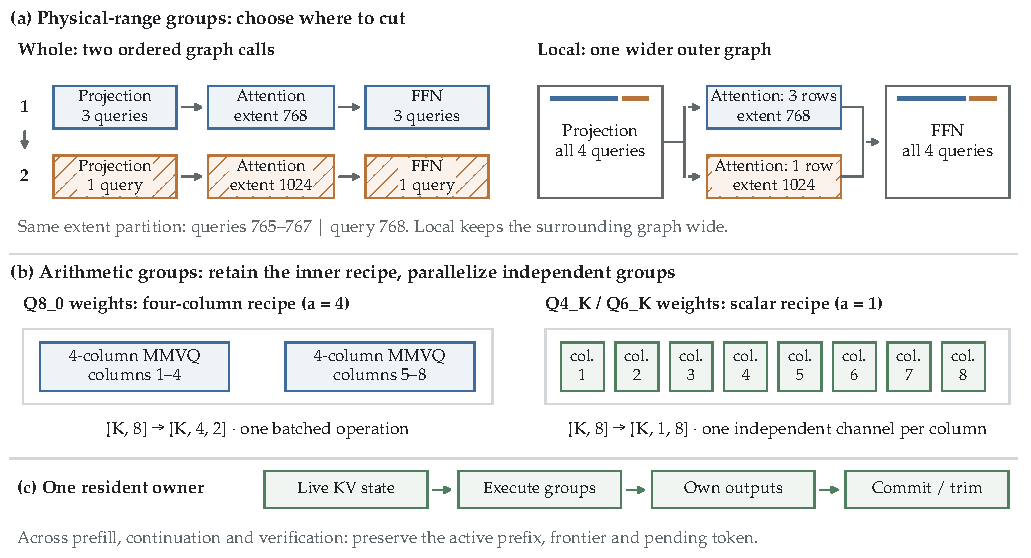
\includegraphics[width=\textwidth]{figures/execution_method.pdf}
\caption{Two choices in reference-compatible execution. Whole execution splits the complete graph into compatible query groups; Local execution confines these cuts to attention and retains wider outer work. The projection, attention and feed-forward blocks repeat across transformer layers. Separately, GPU packing exposes independent arithmetic groups while preserving their inner computation: four columns for the affected CUDA Q8 path and one column for the mixed Q4\_K/Q6\_K path. Physical-extent groups and arithmetic groups serve different constraints. Requested outputs and commit/trim operations share one resident target/KV owner.}
\label{fig:execution_method}
\end{figure*}

\subsection{Expose independent arithmetic groups to the GPU}
\label{sec:recipes}
A wider projection is useful only if its inner computation remains compatible. Let $X\in\mathbb{R}^{K\times q}$ contain $q$ query columns and let $a$ be the native arithmetic group width selected by the recipe. For $q=ag$, a view exposes the independent group index:
\begin{equation}
 \widetilde X_{k,c,j}=X_{k,aj+c},\quad
 \widetilde X\in\mathbb{R}^{K\times a\times g}.
 \label{eq:packing}
\end{equation}
The backend broadcasts the shared weights across $g$ groups and retains the computation within each group. A final view restores logical column order. Eligible shapes and layouts are checked before this mapping; tails use their validated native path.

\subsubsection{CUDA Q8}
For the affected Q8\_0 projections with F32 input, $a=4$ retains the small-column MMVQ computation identified in Section~\ref{sec:reference}. The backend-loop4 control quantizes the input and invokes that specialization for successive groups and the supported tail. Packing uses $[K,4,g]$ views to replace successive backend invocations with one grouped operation. The GPU executes the groups independently while each retains the four-column reduction organization.

A $k=3$ speculative transaction requests at most four target positions, so its verification does not enter the multi-group packing route. Wider prompt work can still use packing. A $k=7$ transaction can request eight positions and expose two groups. Draft prefill width is an independent application parameter.

\subsubsection{Mixed Q4\_K/Q6\_K}
The 32B extension preserves scalar-column computation for the affected Q4\_K and Q6\_K projections, giving $a=1$. Its graph-level control creates scalar-column views, matrix operations and concatenations. Grouping maps the same columns to $[K,1,q]$ and executes them as independent channels. The original per-type dot functions, activation quantizer and accumulation organization are retained. This extends the typed recipe while leaving the Q8 four-column rule intact. Full-model service comparisons use the graph-level scalar-column control; native-operator controls additionally examine the cost of its implementation.

\subsubsection{Vulkan}
The Vulkan mapping retains F32 activations for the affected Q8 projections and dispatches independent column tiles across the GPU grid. In attention, the p021 QK specialization is extended across query workgroups to retain its scalar reduction; AV uses each group's required physical range and qualified stride/dispatch. Recipe selection is phase-specific: the original prompt producer retains its arithmetic, while continuation and verification use the corresponding projection and attention paths. The same physical-prefix planning interface supports two-query verification and wider known-query append, with backend-specific arithmetic beneath it.

\subsection{Carry logical outputs and state across phases}
Prefill, ordinary continuation and verification operate on one resident target/KV owner. A phase transition selects the appropriate recipe and plan while retaining this state. Output reservation specifies storage capacity; the original requested-row mask determines which vectors the call must produce. Table~\ref{alg:plan} summarizes the phase execution.

After each native call, the executor synchronizes and copies its requested vectors into logical output slots before later calls can reuse the scratch buffer. A commit can then select the frontier of the accepted prefix even when a later physical row was rejected. Trimming updates active KV and the logical frontier together. The pending-token record preserves an emitted correction or bonus token until the next phase materializes it, including native cap and end-of-generation behavior. Reset restores the declared initial state; a failed native call invalidates the partially updated owner.

\begin{table}[t]
\centering\footnotesize
\caption{Execution of one reference-derived phase.}
\label{alg:plan}
\begin{minipage}{\columnwidth}
\textbf{Input:} resident state $S$, phase $p$, known rows $Q$ and original requested-row mask $O$.
\begin{enumerate}[leftmargin=1.6em,itemsep=2pt,topsep=4pt]
\item Select the arithmetic recipe from phase and operator descriptors.
\item Check capacity, cache ownership and recipe support; extract each row's physical extent.
\item Form adjacent compatible groups and place whole-graph or attention-local cuts.
\item Apply the supported arithmetic-group packing.
\item Execute native calls in logical order with the original output requests; own requested vectors before scratch reuse.
\item Commit or trim using the owned frontier and pending-token record.
\item Retain the updated owner on success; invalidate it after a failed native call.
\end{enumerate}
\end{minipage}
\end{table}

The argument for Eq.~\eqref{eq:contract} starts from state that matches the reference after the same logical phase history. The recipe must preserve the required outputs and state update for each native group; output ownership and commit/trim must retain the corresponding logical state for the next phase. Under these conditions, induction over groups and phase boundaries preserves the reference relation. Native replays and full-model state checks test these premises in the implemented deployments. Qualification uses independent-reference replay and heavy state capture; service measurements include planning, synchronization, output copies and state updates.

\section{Implementation and Evaluation Design}
\label{sec:eval}
\subsection{Implementations and controls}
We implement the phase planner, attention cuts, typed projection grouping and resident state owner in a pinned llama.cpp/ggml runtime~\cite{records}. CUDA deployments use an RTX 5070 Ti Laptop GPU on Windows and an RTX A5000 on Linux; Vulkan uses an Intel Arc B570. The model families are Qwen3, Llama and SmolLM2~\cite{qwen3,llama3,smol}. Every deployment fixes its reference from the model, tokenizer, prompt producer and numerical modules before evaluating the candidate. The Linux reference and candidates are rebuilt from source, including their CUDA, CPU and base numerical modules.

The evaluated profile uses one dense, nonwrapping sequence, F16 KV, greedy generation and non-flash attention. Known-query calls contain up to 32 positions. The main natural-request studies use context capacity 1024; Vulkan append experiments also use capacity 4096. The Qwen target/draft pairs use Qwen3-8B or 14B with Qwen3-0.6B; the Llama pair uses 8B/1B. Supplement~S1 specifies the producers and numerical qualification; Table~\ref{tab:panels} summarizes the timing designs.

\begin{table*}[t]
\centering\footnotesize\tighttable
\caption{Evaluation panels. A root is one task input; repeated timings retain that root identity. Counts give measured requests or operations, followed by separate warmups. The two Qwen service panels and their factorials reuse the same 16 roots.}
\label{tab:panels}
\begin{tabularx}{\textwidth}{@{}L{2.22cm}L{2.48cm}L{2.62cm}L{2.24cm}Y@{}}\toprule
Question & Deployment & Comparison & Input / repeats & Measured / warm\\\midrule
Component attribution & A5000; Qwen3-8B, 14B & Whole/local $\times$ loop4/packed & 16 roots; 4 balanced rows & $256/32$ per model\\
Natural-request value & A5000; Qwen3-8B, 14B & Four target-only; two speculative & 16 roots; 4 sessions & $384/48$ per model\\
Family transfer & A5000; Llama-8B & Same six controls & 12 roots; 4 sessions & $288/48$\\
Mixed quantization & A5000; Qwen3-32B & Six scalar-loop/grouped paths & 4 roots; 4 rounds & $96/96$\\
Boundary geometry & B570; SmolLM2-1.7B & Scalar, whole and local append & 12 fixed cells; 3 repeats & $108/108$\\
Equal-work width & Windows RTX; Qwen3-8B & One q8 call / two q4 calls & 4 fixed origins; paired repeats & $128/32$\\
Live proposal width & Windows RTX; Qwen3-8B & Whole/local $\times$ loop4/packed $\times$ k3/k7 & 16 roots; 8 balanced rows & $1024/128$\\\bottomrule
\end{tabularx}
\end{table*}

We denote whole-graph and local-attention cuts by W and L, and backend-loop4 and independent-group packing by L4 and P. The loop4 control quantizes activations once and invokes the reference dot computation in the backend. M is ordinary generation and loads only target resources. D4 is speculative generation with draft prefill microbatch four; its proposal count is $k=3$ unless stated otherwise. D4 specifies draft prefill, $q$ counts target query rows, and Q8\_0 specifies weight quantization. All controls receive the same applicable residency, graph-reuse and numerical improvements.

\subsection{Numerical observations and timing boundaries}
Numerical qualification compares each requested full vocabulary vector and active KV state against repeated independent reference runs. Forced-prefix references supply the target values for speculative branches, and autonomous references supply the emitted-token and stopping endpoints. Tests exercise prefill, continuation, boundary crossings, acceptance and rejection, trim, pending tokens, native end of generation, caps and reset. Heavy observers run separately from clean timing; clean runs retain endpoint, transaction-trace, module-identity and physical-work checks.

Natural requests use pinned APPS and MATH inputs~\cite{apps,math}. Linux Qwen experiments reuse the 16 Windows task records with separately established deployment references. Llama uses 12 roots selected after excluding previous project exposure. The live-width panel uses another 16 roots; its equal-work diagnostic uses one APPS and three GSM8K origins~\cite{gsm8k}. Supplement~S1 gives input, warmup and order details.

Resident-service time includes reset, planning, target and draft execution, sampling, state bookkeeping, synchronization and requested-output copying. Separate worker clocks include model loading and warmup. Vulkan append and equal-work width timings start from prepared state and include the specified execution and output copying. These operation timings exclude the separately recorded state preparation.

\subsection{Paired estimates}
For method $A$, root $r$ and session $s$, let $t_{rsA}$ be resident-service time. Our main effect is the ratio of totals,
\begin{equation}
 \rho_{A/B}=\frac{\sum_{r,s}t_{rsA}}{\sum_{r,s}t_{rsB}}.
 \label{eq:ratio}
\end{equation}
Time reduction is $1-\rho$. We compare the candidate with every fixed control; the fastest measured M provides a descriptive application summary. Paired-root bootstrap resampling keeps all arms and sessions of each sampled root together. Application and factorial panels use 10,000 draws and 99\% percentile intervals, applying a Bonferroni adjustment across five predeclared comparisons. Four-arm Williams orders balance positions and directed neighbors in the factorials, which isolate cut and projection effects. The service panels use partial six-arm order balance.

The live-width panel uses eight Williams rows and 98.75\% intervals for four primary width contrasts; its secondary fixed-k7 contrasts form a separate family. Intervals describe variation across the tested roots under the observed sessions. Fixed structural cells and four-root pilots are reported with their observations, without population intervals. Supplement~S3--S4 gives the complete estimands and reconstruction inputs.

\section{Results}
\label{sec:results}
\subsection{Reference observations are preserved}
All requested full-vector and active-state comparisons pass at the qualified transaction boundaries. On Linux, the Qwen/Smol deployment compares 6,740 full vocabulary vectors and 4,784 active-state records across geometry, natural requests and terminal cases. Both model families pass all four target-only cut/projection combinations and both speculative paths. Qwen's grouped-query attention has 128-dimensional heads; Smol's multi-head attention has 64-dimensional heads. The qualified arithmetic recipes preserve the reference observations across both structures.

The Llama transfer uses its own family reference. On Vulkan, combined arithmetic and physical-range repair clears the full-vector differences left by arithmetic repair alone, including the 99 committed differences described in Section~\ref{sec:reference}. The 32B mixed-Q4 extension qualifies all six paths and 60 geometry cases. Eight-query qualification additionally checks all requested rows, boundary crossings, rollback, frontier ownership and pending/terminal transitions. Supplement~S1 records the observation counts and boundaries. The clean timing runs then check the corresponding endpoints and execution traces while measuring the qualified implementation.

\subsection{Packing and local cuts contribute at different scales}
\label{sec:factors}
The balanced Qwen experiments cross W/L attention cuts with L4/P projections while fixing the draft policy, input tasks and proposal count. Each of the four speculative paths is measured in the same panel. Figure~\ref{fig:factorial} separates the two component effects.

\begin{figure*}[t]
\centering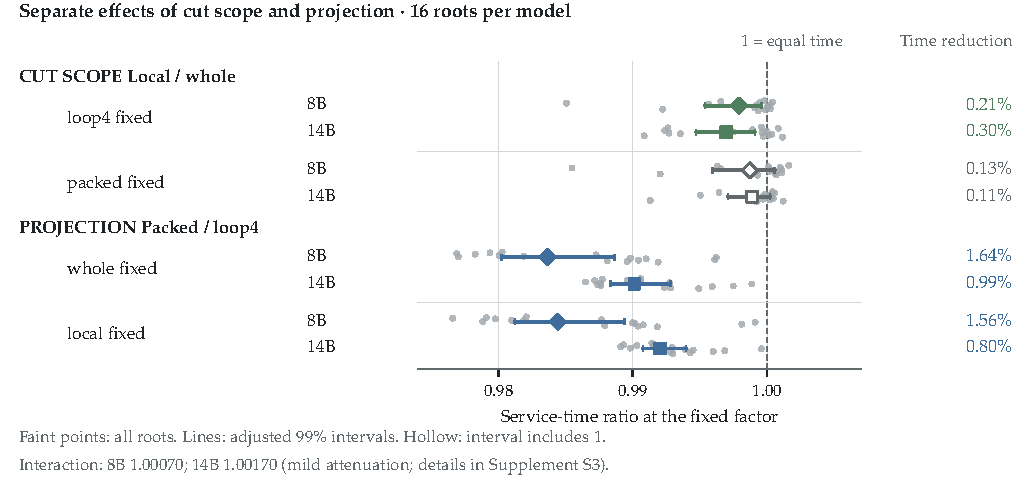
\includegraphics[width=\textwidth]{figures/factorial.pdf}
\caption{Component attribution in balanced A5000 experiments. Points show the 16 task-root ratios; diamonds (8B) and squares (14B) give ratios of total resident-service time. Segments are 99\% paired-root intervals from the five-comparison family. Hollow markers identify intervals that include 1. Projection comparisons fix cut scope; cut comparisons fix projection. The fifth estimand is the interaction in Supplement~S3.}
\label{fig:factorial}
\end{figure*}

Packing reduces service by 1.64\% with whole cuts and 1.56\% with local cuts at 8B, and by 0.99\% and 0.80\% at 14B. The backend-loop4 baseline already moves the loop out of the graph and shares activation quantization, so these differences measure the remaining independent-group packing increment.

Local cuts reduce service by 0.21\% and 0.30\% at fixed loop4 for 8B and 14B. At fixed packing, the reductions are 0.13\% and 0.11\%, with intervals containing 1. The equal-root interactions are 1.000696 and 1.001703, indicating slight attenuation when the components are combined.

\subsubsection{Typed extension to mixed quantization}
For Qwen3-32B, grouping retains the scalar-column Q4\_K and Q6\_K arithmetic and schedules independent columns as channels. Over four roots and four rounds, ordinary grouped execution uses 5.62\% less service with whole cuts and 5.61\% less with local cuts than the graph-level scalar-column loop. All 16 matched pairs improve in each comparison.

A subsequent operator study adds a backend-internal scalar loop: the grouped/backend-loop geometric ratio is 0.8528 over four exposed tensor cells, with mixed paired directions in Q6\_K/q4. Supplement~S3 presents both baselines and all observations. The completed service comparison measures the graph-level grouping implementation; the stronger backend comparison currently supplies operator evidence.

\subsection{Boundary geometry determines the opportunity for local cuts}
\label{sec:geometry}
In the natural 8B factorial, only 20 of 2,224 logical verification cycles require an extra whole-graph boundary split. Local execution uses 2,224 verification graphs; whole execution uses 2,244 for the same target rows. The affected-cycle frequency is 0.899\%. Most verification calls therefore offer no surrounding graph work for local cuts to recover (Fig.~\ref{fig:vulkan}a).

\begin{figure*}[t]
\centering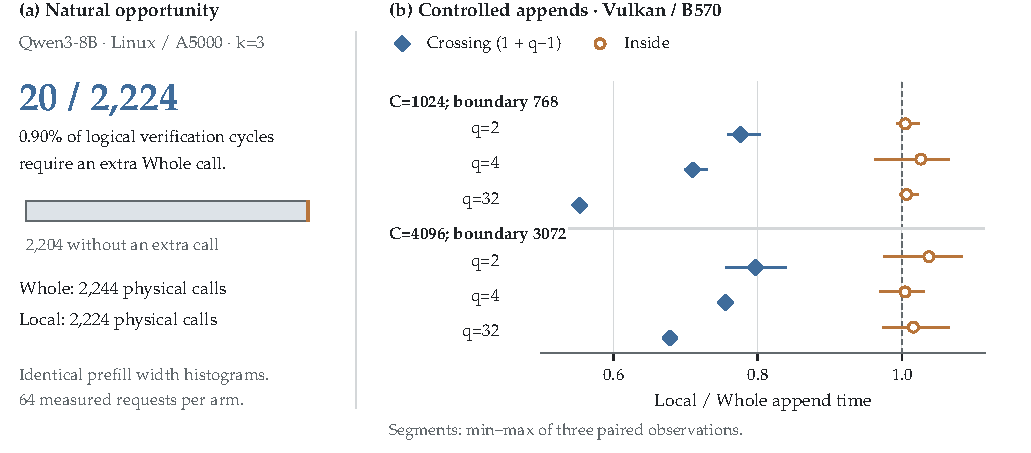
\includegraphics[width=\textwidth]{figures/geometry_opportunity.pdf}
\caption{Where local cuts can help. (a) Natural Qwen3-8B verification on A5000: 20 of 2,224 cycles require an additional whole-graph split, yielding 2,244 whole versus 2,224 local graphs for equal target rows. This is a count of opportunities. (b) Controlled B570 appends at C1024 and C4096: filled markers show boundary crossings and hollow markers their inside controls. Ratios compare local with whole append time; ranges are the minimum and maximum of three paired observations. The two panels measure different quantities.}
\label{fig:vulkan}
\end{figure*}

% Declare the next wide result figure here to avoid a late float.
\begin{figure*}[t]
\centering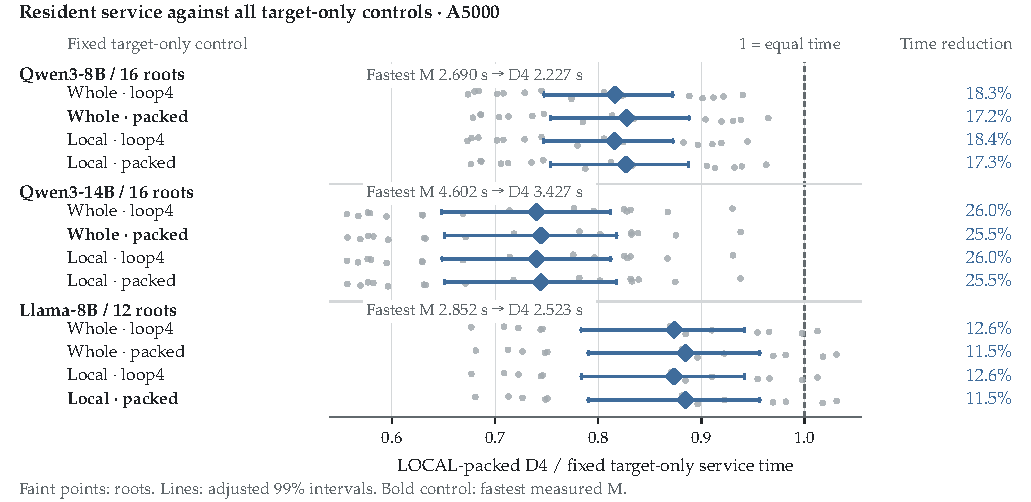
\includegraphics[width=\textwidth]{figures/service_controls.pdf}
\caption{Complete resident-service application comparisons on A5000. Faint points retain all root ratios; diamonds compare LOCAL-packed D4 with each fixed target-only M. Segments are 99\% paired-root intervals from a five-comparison family: the four M comparisons shown here and the W-L4-D4 comparison. Headers give the fastest fixed-M and D4 mean times. Qwen panels share 16 roots; Llama has 12. Table~S1 gives all six arm means.}
\label{fig:service}
\end{figure*}

Controlled Vulkan appends expose the mechanism more directly. We place a call one row before a physical boundary and append $q=2$, 4 or 32 known positions. Whole execution splits the graph as $1+(q-1)$, whereas local execution splits only attention and keeps the surrounding operators wide. Across the six crossing cells at capacities 1024 and 4096, local execution takes 20.34\%--44.68\% less append time. The matched inside controls take approximately 0.43\%--3.74\% more time. Capacity and active-prefix region change together in these cells.

The shape of the split matters. Earlier q32 cells with $16+16$ whole-graph splits included cases favoring whole execution; their complete observations remain in Supplement~S5. Natural-prefix AUTO studies also found little advantage over a whole-graph implementation that rechunks after a boundary. Together, these results explain the two scales in Fig.~\ref{fig:factorial}: local cuts can recover substantial work in a crossing call, while their request-level contribution depends on how often such calls occur.

Packing has a different opportunity. At $k=3$, verification occupies at most four rows and does not enter the wide Q8 packing route. Native execution records locate that route in prefill. Its measured service contribution therefore comes from preserving reference arithmetic while grouping wider known-query work in that phase.

% Declare this wide float early so it stays beside the results it explains.
\begin{figure*}[t]
\centering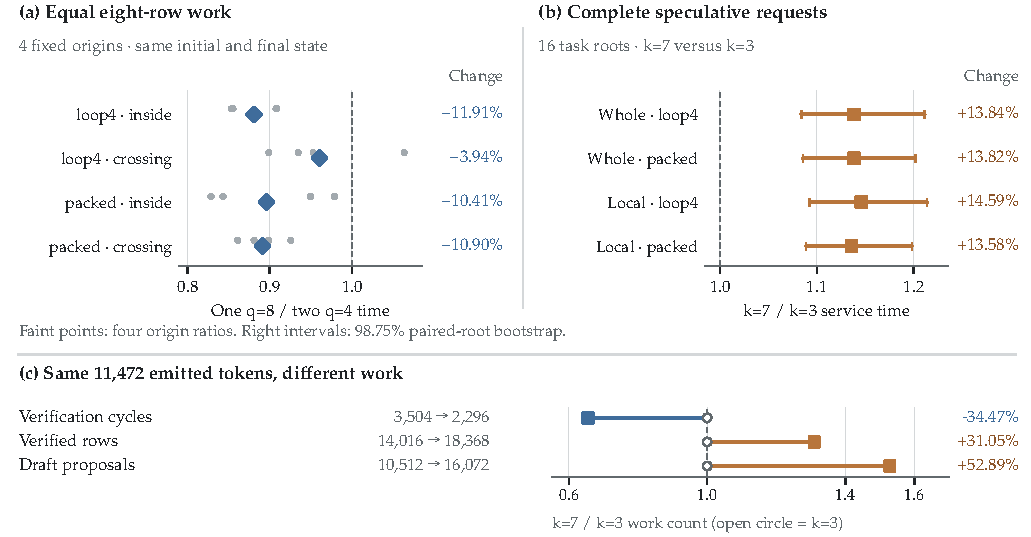
\includegraphics[width=\textwidth]{figures/width_tradeoff.pdf}
\caption{Execution efficiency and live workload. (a) One $q=8$ operation versus two $q=4$ operations from identical state, with the same eight known tokens and all eight requested outputs; faint points retain four development origins. (b) Separate live $k=7$/$k=3$ service comparisons over 16 roots and eight balanced rows, with 98.75\% adjusted intervals. Both widths reserve eight outputs. (c) Work per arm for the same 11,472 emitted tokens: verification cycles fall from 3,504 to 2,296, verified rows rise from 14,016 to 18,368, and draft proposals rise from 10,512 to 16,072.}
\label{fig:width}
\end{figure*}

\subsection{Compatible parallel verification delivers application gains}
\label{sec:application}
Figure~\ref{fig:service} compares complete resident requests with every fixed target-only implementation. LOCAL-packed D4 reduces service relative to all four M controls in each Linux deployment. Against the fastest measured fixed M, mean request time changes from 2.6898 to 2.2269\,s for Qwen3-8B, from 4.6022 to 3.4268\,s for Qwen3-14B, and from 2.8515 to 2.5230\,s for Llama-8B: reductions of 17.21\%, 25.54\% and 11.52\%. The adjusted intervals support each fixed-M comparison.



These gains are the value of the complete speculative application using reference-compatible target execution. Whole-graph execution also supports that application. The independent contributions of packing and cut placement are the smaller effects measured in Section~\ref{sec:factors}.

The 14B improvement persists beyond the resident timer. Its measured-request burst takes 294.632\,s for the fastest fixed M and 219.405\,s for LOCAL-packed D4. Including model loading, integrity checks, primers and the requests, native-worker time falls from 662.546 to 594.559\,s, a 10.26\% reduction. Llama's resident requests improve, but its short worker workload favors M after initialization is included. The Windows Qwen3-8B study separately reports 29.11\% less resident time and 26.00\% less worker time; the Linux Qwen studies reuse the Windows task records with separate references and measurements. Supplement~S2 gives the complete costs.

On the 32B mixed-Q4 panel, ordinary grouped generation is fastest; grouped D4 takes 14.00\% more resident time. In the B570 resident pilot, local verification halves the occupied target-graph count relative to the earlier scalar speculative path, but draft work leaves the complete speculative request slower than ordinary generation.

\subsection{Wider execution and the cost of live work}
\label{sec:width}
The eight-query implementation retains the reference arithmetic and supports $k=7$ proposals plus the pending position. We evaluate physical execution width and live proposal width with separate comparisons (Fig.~\ref{fig:width}).



On the Windows RTX, one q8 call uses 3.94\%--11.91\% less aggregate operation time than two q4 calls across the four fixed method/geometry cells. A matched-history A5000 diagnostic on one exposed origin reports q8/q4-pair geometric ratios of 0.9904 and 0.9781 for loop4, and 0.9370 and 0.9476 for packing. Each A5000 cell has four process clusters; loop4 includes mixed process-level directions. Supplement~S4 retains these observations and the separate live pilot.

In live generation, however, k7 changes the work. Per arm, verification cycles fall from 3,504 to 2,296, while verified rows rise from 14,016 to 18,368 for the same 11,472 emitted tokens. Acceptance among inspected proposals changes little, from 87.47\% to 87.93\%, but accepted proposals as a fraction of all proposals fall from 75.42\% to 56.94\%. Longer proposals spend more work on suffixes that are not consumed.

Consequently, k7 takes 13.58\%--14.59\% more complete service time than k3 across the four methods. For LOCAL-packed, the additional 24.897\,s over 128 requests consists chiefly of 13.567\,s more verification and 13.224\,s more draft proposal, offset by 2.792\,s less draft synchronization. Output copying adds 0.252\,s; the remaining phases close the balance.

The disjoint phase account is
\begin{equation}
 T_{\mathrm{spec}}=T_{\mathrm{target}}+T_{\mathrm{draft}}+T_{\mathrm{state/output/host}}.
 \label{eq:cost}
\end{equation}
The equal-work panels show lower aggregate cost for wider execution. In live generation, the additional target and draft rows outweigh that saving, leaving k3 with the lower complete cost.

\section{Discussion and Related Work}
\label{sec:related}
\subsection{Preserving numerical behavior during optimization}
Batch-invariant inference controls reduction choices in normalization, matrix multiplication and attention~\cite{thinkingmachines}. Taming reconstructs cuBLAS arithmetic, enforces specified reduction order during lowering and statically checks compiled kernels~\cite{taming}. Our experiments trace these numerical dependencies through a quantized runtime's physical attention range, backend arithmetic and placement, and producer/state boundary.

The public \texttt{llama\_reproducible} implementation uses the small-column quantized path~\cite{loop4code}. We retain backend-loop4 as a direct performance control. The packing experiment asks what remains to be gained by exposing its independent groups to the GPU; the factorial design separates that change from attention-local cuts. The mixed-Q4 extension applies the same construction with scalar-column inner arithmetic and its own stated control.

\subsection{Deterministic engines and speculation}
Vosti relates engine state and cache behavior to kernel properties through formal determinism contracts~\cite{vosti}. LLM-42 combines a consistent verifier execution with verification and state repair~\cite{llm42}. CoRun isolates prefill and uses fixed-shape batched decode for deterministic service~\cite{corun}. Our plans combine offline arithmetic qualification with live physical-range and phase requirements, permitting both whole-graph cuts and attention-local cuts within a wider graph.

Speculative decoding and sampling reduce target invocations by verifying proposed tokens together~\cite{leviathan2023,chen2023}. Their distributional arguments and our numerical target address different properties: the latter compares full finite-precision vectors and active state on the evaluated prefixes. HeteroSpec uses contextual heterogeneity to allocate verification effort~\cite{liu2026heterospec}. Proposal policy remains an application choice here; reference-compatible execution supplies the target work that the policy requests.

\subsection{Scope and deployment choices}
The implementation covers a dense, nonwrapping cache, one sequence, F16 KV and non-Flash attention. Its guards make those assumptions explicit. Paged or wrapped caches, additional KV types and fused attention require corresponding geometry extraction and native arithmetic recipes. The two backends already illustrate why the recipe is hardware-specific: identical logical tensors can invoke different activation, reduction and placement choices.

Whole and Local satisfy the same numerical target while exposing different amounts of outer-graph parallel work. Their relative cost depends on boundary frequency and the work outside attention; packing contributes separately. Choosing an application policy also requires the complete cost of draft computation, target verification, output handling and state maintenance.

\Needspace{20\baselineskip}
\section{Conclusion}
Parallel work can be reorganized under a fixed quantized reference by preserving its physical attention ranges, native arithmetic and logical state transitions. Native interventions identify these dependencies before the runtime uses them to derive query groups. Whole and Local place the cuts at different scopes; arithmetic packing exposes independent groups to the GPU while retaining their inner computation. Explicit output ownership carries the resulting state across phases.

CUDA and Vulkan validation checks this construction against full target vectors and active KV. Controlled comparisons quantify the incremental effects of packing and local cuts. Complete-request measurements identify where compatible speculation wins and where additional draft or verification work offsets the saved target time.

\section*{Acknowledgments}
OpenAI ChatGPT and Codex assisted with implementation and analysis tools, manuscript drafting and editing, and figure code. The author is responsible for the scientific content and final approval.
% IEEEtran-provided break balances the final reference columns.
\IEEEtriggeratref{4}
\bibliographystyle{IEEEtran}
\bibliography{references}
\label{lastmainpage}
\end{document}

